%! TEX root = part6.tex
% the main TeX file which is intended to compile, :VimtexReload after adjustment
% :h vimtex-tex-root
\documentclass[../gbr_teknik.tex]{subfiles}
% \includeonlyframes{current}
% \setbeameroption{hide notes} % Only slides
% \setbeameroption{show only notes} % Only notes
\setbeameroption{show notes on second screen=right} % Both

\begin{document}

\begin{frame}[mytitle=center,c,mybg=bglight3,light]
	\frametitle{Tugas Kelas}
	\rtxt{digiPH_red}{digiPH_white}{
		Buatlah gambar \huge pandangan atas dan potongan dari depan \normalsize untuk benda ``Dudukan Penutup'' di bawah ini pada kertas A4. Cantumkan tanda pengerjaan. Pandangan depan sesuai tanda anak panah.
	}
	\limg{tugas_tanda_pengerjaan}
\end{frame}

\begin{frame}[mytitle=standard,c,mybg=bglight2,light]
	\frametitle{Tanda Pengerjaan}
	\begin{center}
		\Large Materi Gambar Teknik Mesin
	\end{center}\end{frame}

\begin{frame}[mytitle=standard,t,mybg=bglight3,light]
	\frametitle{Tujuan Pembelajaran}
	Setelah mempelajari materi ini, mahasiswa mampu:
	\begin{itemize}
		\item Menyebutkan fungsi tanda pengerjaan
		\item Merencanakan tanda pengerjaan pada gambar kerja
		\item Menggunakan tanda pengerjaan pada gambar kerja
	\end{itemize}
\end{frame}

\begin{frame}[mytitle=standard,t,mycolor=digiPH_uniblue,light]
	\frametitle{Pengertian Tanda Pengerjaan}
	\begin{itemize}
		\item Tanda pengerjaan digunakan untuk menunjukkan kualitas permukaan benda kerja
		\item Berkaitan dengan:
		      \begin{itemize}
			      \item Gesekan
			      \item Pelumasan
			      \item Keausan
		      \end{itemize}
		\item Dicantumkan dalam gambar teknik agar teknisi memahami spesifikasi permukaan
	\end{itemize}
\end{frame}

\begin{frame}[mytitle=standard,t,mycolor=digiPH_white,light]
	\frametitle{Fungsi Tanda Pengerjaan}
	\begin{itemize}
		\item Menentukan tingkat kehalusan/kekasaran permukaan
		\item Menjadi acuan proses produksi
		\item Menghindari kesalahan pengerjaan
		\item Menjamin kualitas produk sesuai desain
	\end{itemize}
\end{frame}

\begin{frame}[mytitle=standard,t,mycolor=digiPH_white,light]
	\frametitle{Simbol Dasar Tanda Pengerjaan}
	\begin{itemize}
		\item Terdiri dari dua garis membentuk sudut 60°
		\item Perbandingan tinggi garis = 1 : 2
		\item Ditempatkan pada permukaan yang dikehendaki
	\end{itemize}
\end{frame}

\begin{frame}[mytitle=standard,t,mycolor=digiPH_cream,light]
	\frametitle{Tanda Pengerjaan}
	\begin{center}
		
\includegraphics[width=0.7\textwidth]{tanda pengerjaan.png}
	\end{center}
\end{frame}

\begin{frame}[mytitle=standard,t,mycolor=digiPH_red,dark]
	\frametitle{Jenis Permukaan}
	\begin{itemize}
		\item Permukaan dikerjakan dengan mesin
		\item Permukaan bebas (boleh dikerjakan metode apa saja)
		\item Permukaan tidak boleh dikerjakan
	\end{itemize}
\end{frame}

\begin{frame}[mytitle=standard,t,mycolor=digiPH_red,dark]\begin{itemize}
		\item Tidak semua bagian harus diproses mesin
		\item Beberapa bagian harus dipertahankan dimensinya
	\end{itemize}\end{frame}


\begin{frame}[mytitle=standard,t,mycolor=digiPH_ubcblue,dark]\frametitle{Penulisan Tanda Pengerjaan}
	\begin{itemize}
		\item Simbol dasar dapat diberi keterangan tambahan
		\item Berisi:
		      \begin{itemize}
			      \item Nilai kekasaran
			      \item Metode pengerjaan
			      \item Arah pengerjaan
		      \end{itemize}
	\end{itemize}\end{frame}

\begin{frame}[mytitle=standard,t,mycolor=digiPH_cream,light]
	\frametitle{Tanda Pengerjaan Keterangan}
	\begin{center}
		
\includegraphics[width=0.7\textwidth]{tanda pengerjaan keterangan.png}
	\end{center}\end{frame}

\begin{frame}[mytitle=standard,t,mycolor=digiPH_leaf,dark]\frametitle{Kekasaran Permukaan}
	\begin{itemize}
		\item Kekasaran dinyatakan dengan nilai Ra (μm)
		\item Semakin kecil nilai Ra → semakin halus permukaan
	\end{itemize}
\end{frame}

\begin{frame}[mytitle=standard,t,mycolor=digiPH_cream,light]\begin{tabular}{|c|c|}
		\hline
		Ra (μm)  &  Kelas  \\
		\hline
		0,025    &  N1  \\
		0,05     &  N2  \\
		0,1      &  N3  \\
		0,2      &  N4  \\
		0,4      &  N5  \\
		0,8      &  N6  \\
		1,6      &  N7  \\
		3,2      &  N8  \\
		6,3      &  N9  \\
		12,5     &  N10  \\
		25       &  N11  \\
		50       &  N12  \\
		\hline
	\end{tabular}\end{frame}

\begin{frame}[mytitle=standard,c,mycolor=digiPH_white,light]\frametitle{Arah Pengerjaan}
	\begin{itemize}
		\item Menunjukkan arah bekas pengerjaan mesin
		\item Berpengaruh pada:
		      \begin{itemize}
			      \item Gesekan
			      \item Estetika
			      \item Fungsi komponen
		      \end{itemize}
	\end{itemize}\end{frame}

\begin{frame}[mytitle=standard,t,mycolor=digiPH_white,light]\begin{center}
		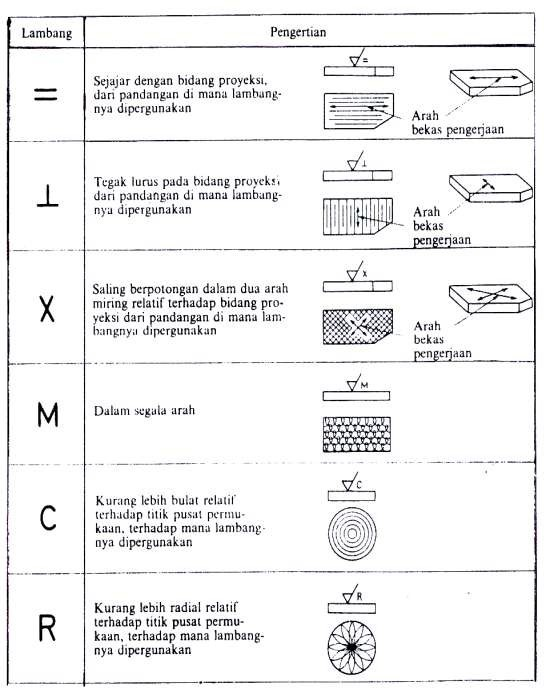
\includegraphics[height=.80\textheight]{../figures/arah pengerjaan.jpg}
	\end{center}\end{frame}

\begin{frame}[mytitle=standard,t,mybg=bglight3,light]\frametitle{Kekasaran Berdasarkan Proses}
	\begin{itemize}
		\item Setiap proses mesin menghasilkan kekasaran berbeda
		\item Contoh:
		      \begin{itemize}
			      \item Grinding → sangat halus
			      \item Bubut → sedang
			      \item Cor → kasar
		      \end{itemize}
	\end{itemize}\end{frame}

\begin{frame}[mytitle=standard,t,mycolor=digiPH_white,light]
	\frametitle{Kekerasan Mesin}
	\begin{center}
		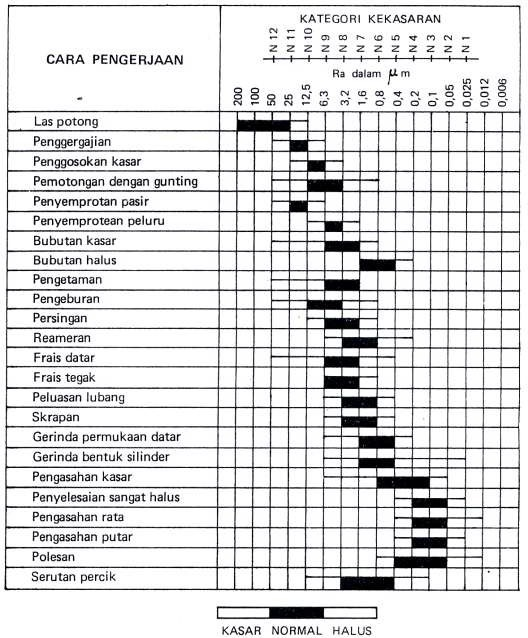
\includegraphics[height=.81\textheight]{../figures/kekerasanmesin.jpg}
	\end{center}
\end{frame}

\begin{frame}[mytitle=standard,t,mycolor=digiPH_gray,light]\frametitle{Kesimpulan}
	\begin{itemize}
		\item Tanda pengerjaan penting dalam gambar teknik
		\item Menentukan kualitas permukaan benda kerja
		\item Membantu teknisi memahami spesifikasi desain
		\item Berpengaruh pada fungsi dan umur komponen
	\end{itemize}\end{frame}




\end{document}
